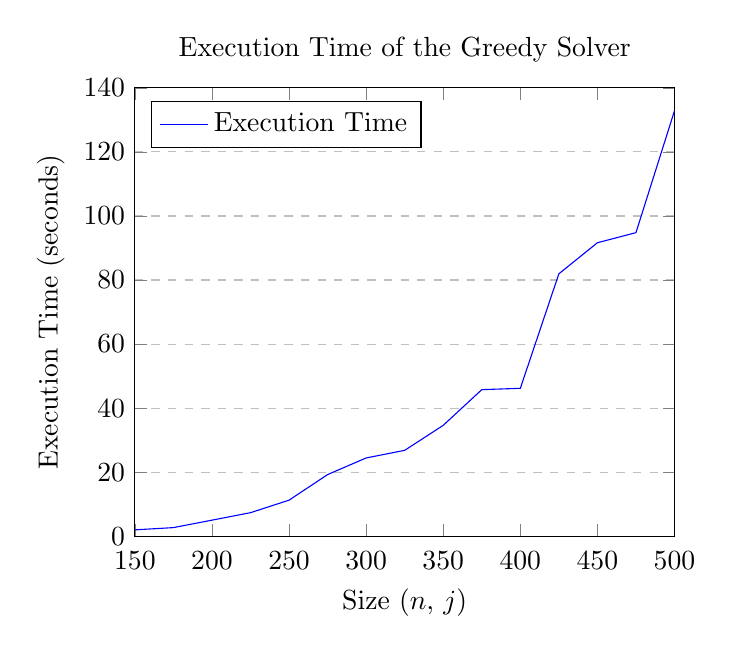
\begin{tikzpicture}
\begin{axis}[
    title={Execution Time of the Greedy Solver},
    xlabel={Size ($n$, $j$)},
    ylabel={Execution Time (seconds)},
    xmin=150, % Set minimum x value to 150
    xmax=500, % Set maximum x value
    xtick={150,200,250,300,350,400,450,500},
    xticklabels={150,200,250,300,350,400,450,500},
    ymin=0, % Set minimum y value to 0
    ymax=140, % Set maximum y value
    ytick={0,20,40,60,80,100,120,140}, % Set y ticks in steps of 20
    symbolic x coords={150,175,200,225,250,275,300,325,350,375,400,425,450,475,500},
    xticklabel style={anchor=base, yshift=-\baselineskip},
    yticklabel style={/pgf/number format/fixed},
    legend pos=north west,
    ymajorgrids=true,
    grid style=dashed,
]
\addplot[
    color=blue,
    ]
    coordinates { % 
    (150,1.98) (175,2.68) (200,5.01) (225,7.34) (250,11.25) (275,19.24) (300,24.43) (325,26.81) (350,34.62) (375,45.76) (400,46.18) (425,81.94) (450,91.64) (475,94.79) (500,132.87)
    };
    \legend{Execution Time}
\end{axis}
\end{tikzpicture}